\begin{flushright} {\tiny {\color{gray} nomenclature.tex}} \end{flushright}
%~~~~~~~~~~~~~~~~~~~~~~~~~~~~~~~~~~~~~~~~~~~~~~~~~~~~~~~~~~~~~~~~~~~~~~~~~~~~~~~~~~~~~~~~~~~~~~~~~~

\begin{center}
\begin{tabular}{lll}
\hline
Symbol & meaning & unit \\
\hline
\hline
$t$ & Time & \si{\second} \\
$x,y,z$ & Cartesian coordinates & \si{\metre} \\
$r,\theta$ & Polar coordinates & \si{\metre},-\\
$r,\theta, z$ & Cylindrical coordinates & \si{\metre},-,\si{\metre}\\
$r,\theta,\phi$ & Spherical coordinates & \si{\metre},-,- \\
${\vec \upnu}=(u,v,w)$ & velocity vector$^{(1)}$  & \si{\metre\per\second}\\
${\vec \upnu}=(\upnu_r,\upnu_\theta,\upnu_z)$ & velocity vector$^{(2)}$ & \si{\metre\per\second}\\
${\vec \upnu}=(\upnu_r,\upnu_\theta,\upnu_\phi)$ & velocity vector$^{(3)}$ & \si{\metre\per\second}\\
${\vec u}=(u_x,u_y,u_z)$ & displacement vector & $\si{\metre}$ \\
$\rho$ & mass density & \si{\kg\per\cubic\metre} \\
$\eta$ & dynamic viscosity & \si{\pascal\second} \\
$\lambda$ & penalty parameter & \si{\pascal\second} \\
$T$ & temperature & \si{\kelvin} \\
${\vec \nabla}$ & gradient operator & \si{\per\metre} \\
${\vec \nabla}\cdot$ & divergence operator & \si{\per\metre} \\
$p$ & pressure & \si{\pascal}\\
$\dot{\bm \varepsilon}({\vec \upnu})$ & strain rate tensor & \si{\per\second} \\
$\dot{\bm \varepsilon}^d({\vec \upnu})$ & deviatoric strain rate tensor & \si{\per\second} \\
$\alpha$ & thermal expansion coefficient & \si{\per\kelvin} \\
$k$ & thermal conductivity & \si{\watt\per\metre\per\kelvin} \\
$C_p$ & Heat capacity at constant pressure & \si{\joule\per\kg\per \kelvin} \\
$H$ & intrinsic specific heat production & \si{\watt\per\kg} \\
$\beta_T$ & isothermal compressibility & \si{\per\pascal}  \\
${\bm \tau}$ & deviatoric stress tensor & \si{\pascal} \\
${\bm \sigma}$ & full stress tensor & \si{\pascal} \\
\hline
\end{tabular}\\
{\tiny (1) Cartesian coordinates;} 
{\tiny (2) Cylindrical coordinates;} 
{\tiny (3) Spherical coordinates.}
\end{center}

\begin{center}
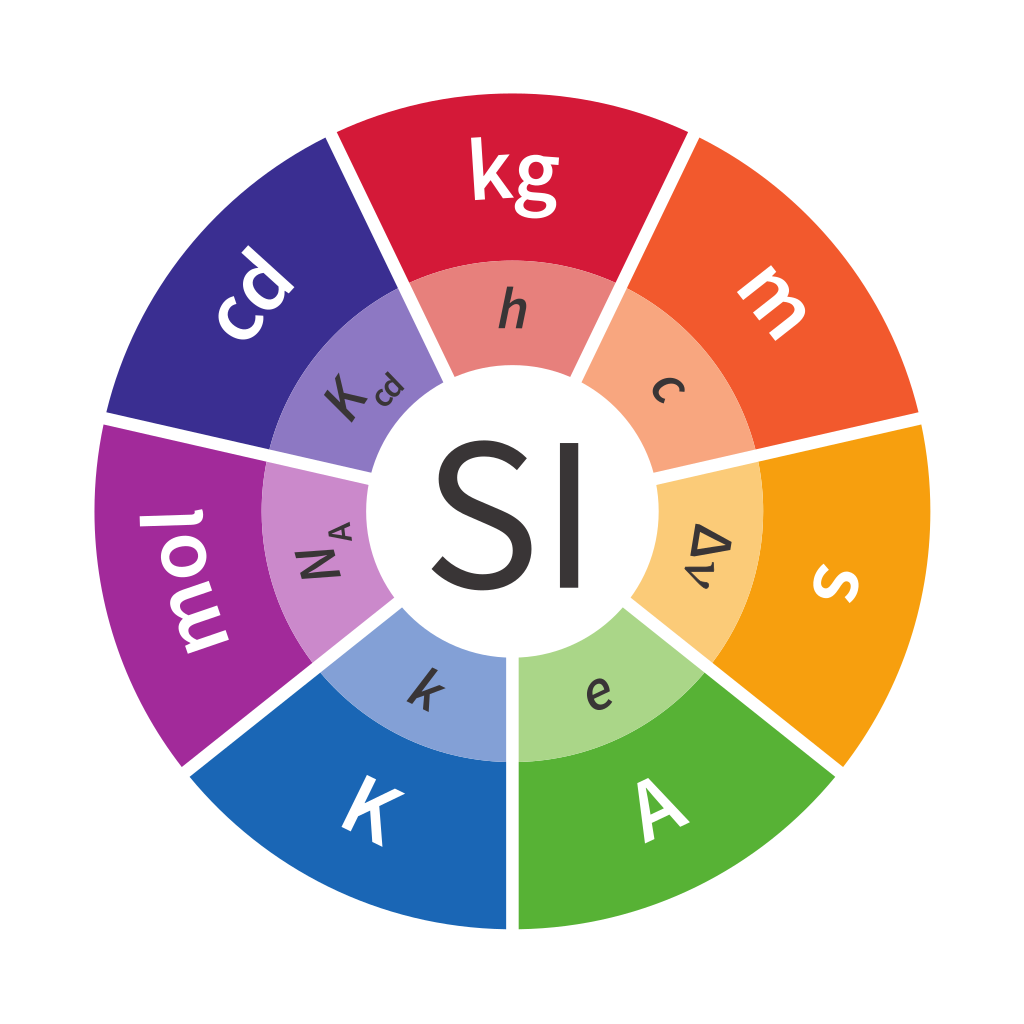
\includegraphics[width=5cm]{images/siunits}\\
{\captionfont Taken from 
Wikipedia\footnote{\url{https://en.wikipedia.org/wiki/International_System_of_Units}}.
The SI logo, produced by the BIPM (International Bureau of Weights and Measures), \\
showing the seven SI base units and the seven defining constants.}
\end{center}

A quick note about units and \LaTeX. This document relies on the {\tt siunitx} 
package\footnote{\url{https://ctan.org/pkg/siunitx}}. For instance, 
$\rho = 3300~\si{\kg\per\cubic\metre}$ is obtained with 
\begin{verbatim}
\rho = 3300~\si{\kg\per\cubic\metre}
\end{verbatim}
or
\begin{verbatim}
\rho = \SI{3300}{\kg\per\cubic\metre}
\end{verbatim}
Note that the {\tt si} command can be used outside of the math environment. 
